%%% Класс документа
\documentclass[a4paper,12pt]{article}

%%% Работа с русским языком
\usepackage{cmap}					% поиск в PDF
\usepackage[T2A]{fontenc}			% кодировка
\usepackage[utf8]{inputenc}			% кодировка исходного текста
\usepackage[english,russian]{babel}	% локализация и переносы
\usepackage{mathtext} 				% русские буквы в формулах
\usepackage{csvsimple}              % for tabular from csv loading
\usepackage{indentfirst}            % indent after sections
%\usepackage{minipage}

%%% Дополнительная работа с математикой
\usepackage{amsmath,amsfonts,amssymb,amsthm,mathtools} % AMS
\usepackage{icomma} % "Умная" запятая: $0,2$ --- число, $0, 2$ --- перечисление

%%% Номера формул
%\mathtoolsset{showonlyrefs=true} % Показывать номера только у тех формул, на которые есть \eqref{} в тексте.
%\usepackage{leqno} % Немуреация формул слева

%%% Шрифты
\usepackage{euscript}	 % Шрифт Евклид
\usepackage{mathrsfs} % Красивый матшрифт

%%% Свои команды
\DeclareMathOperator{\sgn}{\mathop{sgn}}

%%% Перенос знаков в формулах (по Львовскому)
\newcommand*{\hm}[1]{#1\nobreak\discretionary{}
{\hbox{$\mathsurround=0pt #1$}}{}}

%%% Работа с картинками
\usepackage{graphicx}  % Для вставки рисунков
\graphicspath{{images/}{images2/}}  % папки с картинками
\setlength\fboxsep{3pt} % Отступ рамки \fbox{} от рисунка
\setlength\fboxrule{1pt} % Толщина линий рамки \fbox{}
\usepackage{wrapfig} % Обтекание рисунков и таблиц текстом

%%% Работа с таблицами
\usepackage{array,tabularx,tabulary,booktabs} % Дополнительная работа с таблицами
\usepackage{longtable}  % Длинные таблицы
\usepackage{multirow} % Слияние строк в таблице

%%% Теоремы
\theoremstyle{plain} % Это стиль по умолчанию, его можно не переопределять.
%\newtheorem{theorem}{Теорема}[section]
%\newtheorem{proposition}[theorem]{Утверждение}

%\theoremstyle{definition} % "Определение"
%\newtheorem{corollary}{Следствие}[theorem]
%\newtheorem{problem}{Задача}[section]

%\theoremstyle{remark} % "Примечание"
%\newtheorem*{nonum}{Решение}

%%% Программирование
\usepackage{etoolbox} % логические операторы

%%% Страница
\usepackage{extsizes} % Возможность сделать 14-й шрифт
\usepackage{geometry} % Простой способ задавать поля
	\geometry{top=25mm}
	\geometry{bottom=25mm}
	\geometry{left=24mm}
	\geometry{right=24mm}

%%% Колонтитулы
%\usepackage{fancyhdr}
 	%\pagestyle{fancy}
 	%\renewcommand{\headrulewidth}{0mm}  % Толщина линейки, отчеркивающей верхний колонтитул
 	%\lfoot{Нижний левый}
 	%\rfoot{Нижний правый}
 	%\rhead{Верхний правый}
 	%\chead{Верхний в центре}
 	%\lhead{Верхний левый}
 	% \cfoot{Нижний в центре} % По умолчанию здесь номер страницы

%%% Интерлиньяж
%\usepackage{setspace}
%\onehalfspacing % Интерлиньяж 1.5
%\doublespacing % Интерлиньяж 2
%\singlespacing % Интерлиньяж 1

%%% Гиперссылки
\usepackage{hyperref}
\usepackage[usenames,dvipsnames,svgnames,table,rgb]{xcolor}
\hypersetup{				% Гиперссылки
    unicode=true,           % русские буквы в разделареальных установках
    pdfproducer={Производитель}, % Производитель
    pdfkeywords={keyword1} {key2} {key3}, % Ключевые слова
    colorlinks=true,       	% false: ссылки в рамках; true: цветные ссылки
    linkcolor=red,          % внутренние ссылки
    citecolor=green,        % на библиографию
    filecolor=magenta,      % на файлы
    urlcolor=cyan           % на URL
}

%%% Другие пакеты
\usepackage{lastpage} % Узнать, сколько всего страниц в документе.
% \usepackage{soul} % Модификаторы начертания
\usepackage{csquotes} % Еще инструменты для ссылок
%\usepackage[style=authoryear,maxcitenames=2,backend=biber,sorting=nty]{biblatex}
\usepackage{multicol} % Несколько колонок

%%% Шрифты
%\renewcommand{\familydefault}{\sfdefault} % Начертание шрифта


%%% Работа с библиографией
%\usepackage{cite} % Работа с библиографией
%\usepackage[superscript]{cite} % Ссылки в верхних индексах
%\usepackage[nocompress]{cite} %
%\usepackage{csquotes} % Еще инструменты для ссылок


%%% Tikz
\usepackage{tikz} % Работа с графикой
\usepackage{pgfplots} % Работа с pgf
\usepackage{pgfplotstable}

%%% Дополнительные пакеты для tikz
\usepgfplotslibrary{dateplot} % Возможность подписания дат
\pgfplotsset{compat=1.5}

\newcommand{\boldm}[1]{{\boldsymbol{#1}}}

\usepackage{upgreek}

\begin{document}
\begin{center}

    \normalsize{Федеральное государственное автономное образовательное учреждение высшего образования}

    \textbf{НАЦИОНАЛЬНЫЙ ИССЛЕДОВАТЕЛЬСКИЙ УНИВЕРСИТЕТ \\ <<МОСКОВСКИЙ ФИЗИКО-ТЕХНИЧЕСКИЙ ИНСТИТУТ>>}
    \vspace{13ex}

    \textbf{Эссе по защите информации}

    \textbf{<<Атаки протокольного туннелирования>>}
    \vspace{40ex}
\end{center}
\begin{flushright}
    \normalsize{Выполнил: Дурнов Алексей Николаевич \\ студент Б01-009 \\}
\end{flushright}

\vfill

\begin{center}
Долгопрудный, 2023
\end{center}

\thispagestyle{empty} % выключаем отображение номера для этой страницы

\newpage

\tableofcontents{}
\newpage

\section{Введение}

Технологии DPI обеспечивают необходимую видимость и контроль сетевого трафика с помощью независимой от порта идентификации протокола,
когда сетевой поток маркируется протоколом прикладного уровня на основе содержимого пакета. С помощью DPI-систем можно блокировать необходимый трафик.
Существуют атаки на неправильную идентификацию протокола, когда пытаются заставить DPI неверно маркировать соединения.
Разработка систем защиты от блокировок привели к другим побочным проблемам: ограничение на развертывание, низкий уровень QoS и т.д.
Эти проблемы препятствуют к их широкому внедрению.

В данной работе будет представлена классификация систем обхода блокировок.
На примере Tor будут рассмотрены существующие инструменты обфускации соединений и ухода от блокировок.
А также подробно разобран криптографический примитив: форматно-преобразующее шифрование,
которое помогает уклоняться от блокировок, лишь понижая пропусную способность на 16\% по сравнению со стандартными SSH-туннелями.

\section{Классификация систем обхода блокировок}
В целях содествия свободе слова и беспрепятственному обмену информацией в Интернете,
ученые предлагали различные решения для обхода блокировок и борьбы с цензурой на протяжении многих лет.
Попытаемся классифицировать их и перечислить преимущества и недостатки.

\begin{enumerate}

    \item \textbf{Системы на основе прокси-серверов}: К таким системам относятся прокси-сервера, VPN, Tor и т.д.
    В них клиенты передают свой трафик через промежуточные прокси-сервера, которые от имени клиентов подключаются к заблокированным сайтам.
    Подобный подход позволяет легко разворачивать такие системы, однако их также легко детектировать по публичным IP-адрессам прокси-серверов.
    Таким образом, противнику не составляет труда блокировать их сразу же после обнаружения.

    \item \textbf{Системы ложной маршрутизации}:
    Этот метод является перспективным и позволяет клиентам, находящимся под цензурой, получать доступ с помощью обращения к незаблокированных веб-сайтам.
    Запросы содержат скрытую информацию, которая перехватывается и расшифровывается специальными промежуточными маршрутизаторами.
    Эти маршрутизаторы передают запросы и ответы между клиентами заблокированным сайтом, маскируясь за соединением между клиентом и незаблокированном сайтом.
    Примерами таких систем являются Telex, Waterfall of Liberty и SiegeBreaker.
    Блокировка таких систем требует сложных мер, например, изменения политики маршрутизации на уровне всей страны.
    Однако для их функционирования требуется сотрудничество с провайдерами, что может стать препятствием для их развертывания.

    \item \textbf{Системы, основанные на мимикрии}:
    Цензурируемое содержимое в таких системах пытаются закамуфлировать и передать под видом сообщения обычного протокола приложений.
    Например, SkypeMorph помогает получить доступ к заблокированным сайтам, имитируя протокол общения Skype.
    Однако такие протоколы очень легко блокируются, так как тяжело передать все особенности базового протокола.
    Кроме того, их эффективность зависит от скорости протоколов прикрытия. Для Skype выделяется низкие скорости передачи данных,
    что приводит к низкому уровню QoS для просмотра веб-страниц.

    \item \textbf{Системы, основанные на туннелировании}:
    Они полагаются на инкапсуляцию скрытого трафика в сообщениях стандартных прикладных протоколов – например, электронную почту, VoIP, видеопотоки, онлайн-игры и т.д.
    В качестве примеров можно привести SWEET, Covertcast, Delta Shaper, Freewave, CloudTransport, Rook и др.
    Такие системы являются улучшением по сравнению с системами, основанные на мимикрии, поскольку они не имитируют протокольные сообщения,
    а непосредственно используют их в качестве скрытых каналов.
    Они используют все особенности прикрывающего протокола, в то время как цензурируемое содержимое инкапсулируется в полезную нагрузку.
    Это очень сильно затрудняет цензору к их дифференциации от обычных (базовых) протокольных сообщений.
    Таким образом, может потребоваться блокировка всех базовых приложений (таких как электронная почта, облачные сервисы и т.д.), что может привести к масштабным убыткам.
    Однако такие системы всё также плохо обеспечивают QoS.

    \item \textbf{Прочие системы}:
    Существуют и другие системы для борьбы с блокировками, не относящихся ни к одному из выше перечисленных типов.
    Domain fronting использует сторонние серверы, например, Microsoft Azure, для доступа к цензурируемому контенту.
    Запрос к прокси-серверу (скрытому за облачным сервером), скрывается в протоколе HTTPS, который направляется на доменное имя безобидного внешнего интерфейса облачного сервера.
    Этот модуль расшифровывает HTTPS-запрос и направляет его на прокси-сервер.
    Для блокирования таких сервисов противнику может потребоваться заблокировать весь фасадный сервис (например, Microsoft Azure), тем самым
    тем самым блокируя другие сторонние приложения, использующие эту платформу. Разворачивать такие системы не является экономически эффективным.


\end{enumerate}

Теперь посмотрим, какие системы используются на практике и как они взаимодействуют друг с другом.

\section{Tor}

С 2002 года система Tor стала популярной среди пользователей, которые хотят обходить цензуру и общаться анонимно.
Но многие страны пытаются заблокировать доступ к этой системе для своих граждан.
Сначала они добавляли сайт Tor в черный список, чтобы пользователи не могли скачать клиентское ПО.
Затем они использовали все более изощренные методы блокировки:
активно загружался список узлов Tor (также называемых ретрансляторами) с Tor Directory Servers и вносился в черный список,
устанавливались DPI-системы для поиска характеристик связи Tor (например, набор шифров рукопожатия TLS в Tor), а также активное зондирование
(выдача себя за Tor-клиента и подключение к подозрительным серверам для проверки наличия у них Tor-релея).
Tor сообщество не стояло на месте и разрабатывали методы обхода попыток блокировок: Tor Bridges и Pluggable Transports (PTs).

\begin{figure}[h!]
    \begin{center}
        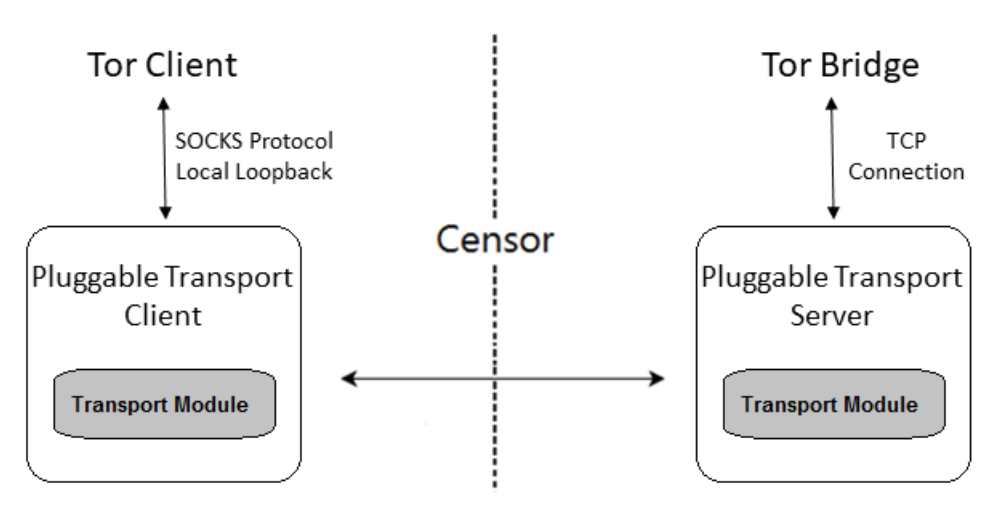
\includegraphics[width = 0.5\textwidth]{tor_pt.png}
        \caption{Устройство Tor соединения с Pluggable Transports}
    \end{center}
\end{figure}

PT являются общей основой для создания и внедрения технологий обхода блокировок.
Они обеспечивают обфускацию соединения между клиентом Tor и мостом, который служит защитой входа в Tor,
таким образом, что оно выглядит как доброкачественное.
PT необходимо установить как на стороне клиента Tor, так и на стороне моста.
PT открывают SOCKS-прокси для клиентского приложения Tor, обфусцирует или иным образом преобразует трафик, прежде чем направить его на мост.
На стороне моста сервер PT выставляет обратный прокси, который принимает соединения от клиентов PT и декодирует обфускацию/трансформацию,
примененную к трафику, перед передачей его реальному приложению моста.
Данные, передаваемые между PT-клиентом и PT-сервером, могут быть зашифрованы, разрезаны на части или иным образом замаскированы,
что делает их труднодоступными для цензора, который может обнаружить данные Tor и заблокировать их.
Преобразование/обфускация данных и обратные операции выполняются транспортными модулями/протоколами обфускации, используемыми PT.
По состоянию на сентябрь 2017 года, доступными и развернутыми протоколами обфускации в браузере Tor являются: obfs3, obfs4, ScrambleSuit, FTE и meek.

\begin{enumerate}

    \item \textbf{Obfs3}: создает дополнительный уровень шифрования поверх TLS-соединения Tor, чтобы скрыть его уникальные характеристики.
    Для обмена ключами шифрования используется неаутентифицированный кастомизированное рукопожатие Диффи-Хеллмана.
    В результате этот протокол подвержен атакам активного зондирования.

    \item \textbf{ScrambleSuit}: протокол, который защищает от атак активного зондирования,
    используя внеканальный обмен секретами и изменение сетевого отпечатка
    (распределение длины пакетов, время между приходами и т.д.). Он может быть заблокирован на основе ``белых списков''.

    \item \textbf{Obfs4}: является логическим развитием ScrambleSuit.
    Была улучшена скорость работы и добавлена мостовая аутентификация,
    за счёт обфускации открытый ключей по технологии Elligator и протокола ntor.
    Он также может быть заблокирован на основе ``белых списков''.


    \item \textbf{Meek}: использует технологию Domain Fronting для ретрансляции Tor-трафика через сторонние серверы.
    (то есть CDN, такие как Microsoft Azure, Google app engine, Amazon CloudFront и другие).

    \item \textbf{Format-Transforming Encryption (FTE)}:
    преобразовывает трафик Tor с помощью регулярных выражений в произвольные форматы стандартных протоколов,


\end{enumerate}

Эти протоколы обфускации можно разделить на две группы:

\begin{enumerate}

    \item \textbf{Протоколы случайных потоков (obfs3, obfs4 и ScrambleSuit)}:
    Обмен данными в этих протоколах осуществляется в виде потоков случайных байтов,
    которые невозможно соотнести ни с одним известным протоколом.
    Данные протоколы включают в себя две фазы: фазу рукопожатия, где ключи обмениваются между участниками,
    и фазу передачи данных, где зашифрованные сообщения передаются с использованием полученных ключей.

    \item \textbf{Структурированные потоковые протоколы (FTE и meek)}:
    пытаются скрыть свою активность, имитируя известные протоколы из "белого списка", такие как DNS и HTTP.

\end{enumerate}

Цензурирующие страны, использующие активному зондирование, могут распознать мосты, использующие obfs3.
Кроме того, протоколы случайных потоков могут быть заблокированы цензором по стратегии "белого списка",
так как их отпечаток не соответствует известным протоколам.
С другой стороны, структурированные потоковые протоколы, имитирующие распространенные протоколы,
устойчивы к блокированию на основе "белых списков", но не защищают от активного зондирования.

Из этих соображений приходит идея сделать установление соединений, уже используя существующее решение - протокол obfs4,
но при этом нужно прятать с помощью туннелирования или мимикрии эти сообщения в протокол,
который обязан быть в ``белом списке'' для работы всех систем. Таким протоколом может выступать DNS.
После установление соединения данные можно передавать всё-также с помощью мимикрии или туннелирования под протокол HTTP.
При этом в сети не будет всплеска DNS траффика, по которому можно будет детектировать данное скрытое соединение.
Но чтобы реализовать подобное, нужно познакомиться с форматно-преобразующим шифрованием FTE.

\section{FTE}

Часть DPI систем используют явно или неявно регулярные выражения для классификации протоколов на прикладном уровне,
поэтому рассмотрим механизмы, позволяющие злоумышленнику принудительно идентифицировать протокол, против любого DPI, основанного на проверке регулярных выражений.
Основная идея заключается в том, чтобы встроить защиту от DPI в схемы шифрования.
Добавим к обычному интерфейсу шифрования возможность принимать на вход регулярное выражение.
Задача этого регулярного выражения определять формат шифротекстов: это означает,
что шифротексты, взятые в виде строк соответствующего алфавита, гарантированно будут соответствовать заданному регулярному выражению.
Такой криптографический примитив называется форматно-преобразующим шифрованием (FTE).
Благодаря правильному выбору регулярного выражения, шифротексты, которые на самом деле несут исходный протокол,
будут классифицироваться DPI как сообщения от другого протокола, по нашему выбору.

Схема FTE состоит из трех алгоритмов: генерация ключа, шифрования и дешифрования.
Генерация ключа работает, как и в обычном шифровании, с выдачей случайно выбранного симметричного ключа $K$.
Входными параметрами функции шифрование $Enc$ являются ключ $K$, формат $\mathcal{F}$ и сообщение $M$,
а выходным параметром всегда является шифротекст $C$ или символ ошибки $\perp$.
шифрование может быть с сохранением состояния, случайном или полностю детерминированным.
Входными параметрами функции расшифрования является ключ $K$, формат $F$ и шифротекст $C$,
а выходным параметром является сообщение или символ ошибки $\perp$.
Формат $\mathcal{F}$ определяет множество $L(\mathcal{F})$, называемое языком формата $\mathcal{F}$.
Любой шифротекст $C$, выводимый функцией шифрования $Enc$, должен быть элементом языка $L(\mathcal{F})$.

Есть схожий примитив шифрование сохраняющий формат (FPE), впервые формализированно Bellare, Ristenpart, Rogaway и Stegers (BRRS).
Главное его отличие от FTE заключается в том, что и открытый текст, и шифротекст были элементами одного и того языка, определенного формата.

FTE должен поддерживать форматы, описываемые регулярными выражениями,
что позволит ``программировать'' форматы и даст FTE те же выразительные возможности, что и DPI системы на основе регулярных выражений.

Для регулярного выражения $\mathcal{F}$ реализация функции шифрования $Enc(K, \mathcal{F}, M)$:

\begin{enumerate}
    \item Шифруем сообщение $M$ с помощью стандартной схемы аутентифицированного шифрования, получая промежуточный шифротекст $Y$.
    \item Рассматриваем $Y$ как число в $\mathbb{Z}_{|L(\mathcal{F})|}$ (в кольце класса вычетов по модулю размера языка).
    \item Применяем кодирующию функцию unrank: $\mathbb{Z}_{|L(\mathcal{F})|} \rightarrow L(\mathcal{F})$.
\end{enumerate}


Для возможности расшифровки требуем, чтобы unrank была биективной функцией с эффективно вычислимой обратной функцией rank:
$L(\mathcal{F}) \rightarrow \mathbb{Z}_{|L(\mathcal{F})|}$.


Одной из ключевых проблем данного решения является эффективная реализация функций rank и unrank,
которые связывают каждую строку языка с ее рангом, то есть позицией в упорядоченном языке.

Goldberg и Sipser разработали эффективный метод ранжирования регулярного языка,
представленного детерминированным конечным автоматом (DFA).
BRRS использовали этот подход для нереализованной схемы FPE для произвольных регулярных языков,
представленных в виде DFA. Однако они также отметили, что не существует асимптотического доказательства
эффективности функций rank и unrank при работе с регулярными выражениями.
Существует стандартные средства для преобразования регулярного выражения в недетерминированный конечный автомат (NFA),
а затем в DFA, но второй шаг приводит к экспоненциальному раздуванию размера состояния.
Такое поведение в худшем случае не является проблемой для FTE, частично потому,
что используемые в DPI типы регулярных выражений специально разработаны для предотвращения увеличения размера в худшем случае.

Авторы алгоритма FTE нашли компромиссный способ выполнения ранжирования строк языка $x \in L$ между временем и памятью,
предварительно вычисляя таблицы для этой цели при условии, что $|x| \leq n$, где $n$ - длина строки, а следовательно и длина выхода $rank_{L}$ и входа $unrank_{L}$.
Сложность предварительной обработки составляет $O(n \cdot |\Sigma| \cdot |Q|)$, где $\Sigma$ - базовый алфавит,
а $Q$ - множество состояний DFA, реализующее регулярное выражение $F$.
С учетом таблиц, сложность функций $rank_{L}$ и $unrank_{L}$ составляет $\Omega(n)$ и $O(n \cdot |\Sigma|)$ соответственно.

\begin{figure}[h!]
    \begin{center}
        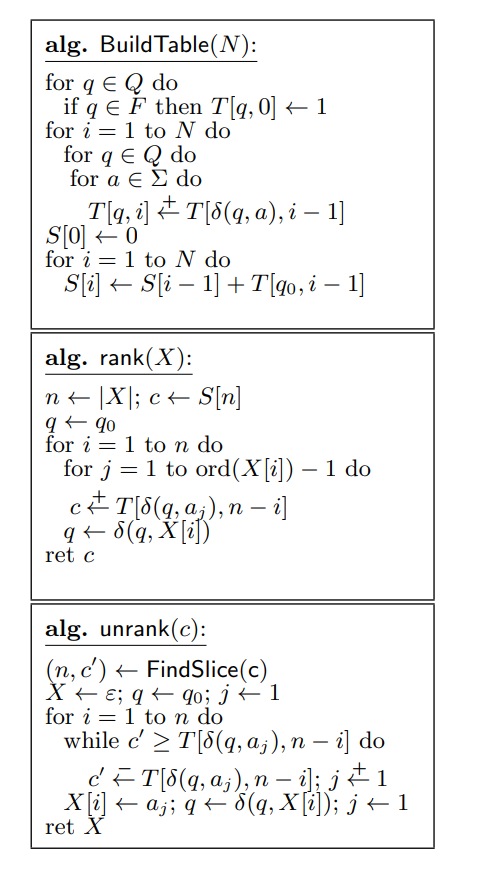
\includegraphics[width = 0.3\textwidth]{algos.png}
        \caption{Возможные реалиазации функций rank и unrank}
        \label{algos}
    \end{center}
\end{figure}

На рис \ref{algos} можно увидеть возможные реализации функций rank и unrank, и вспомогательной функции построения таблицы.

Детерминированный конечный автомат $M$ опредяляется своим конечным множеством сотояний $Q$,
конечным множеством входных символов, называемых алфавитом $\Sigma$, функцией перехода $\delta$: $Q \times \Sigma \rightarrow Q$,
начальным состоянием автомата $q_0 \in Q$ и множеством допустимых состояний $F \subset Q$.

Порядковый номер символа $\alpha \in \Sigma$, записан как $ord(\alpha)$, это позиция символа в лексикографическом порядке элементов $\Sigma$.
$T(q, i)$ - это количество строк длины i, которые заканчиваются в допустимом состоянии при запуске из состояния q.
Так $T(q_0, i)$ - это количество $X \in L$, таких, что $|X| = i$.
$S[i]$ - это количество строк в $L$ длины не более, чем $i - 1$.
Неуказанный алгоритм FindSlice находит наибольшее $l$, такое что $S[l] < c$, и возвращает $n = l + 1$, $c' = c - S[l]$.
Это можно сделать бинарным поиском за $O(\log_2(|S|))$.

Подход ``Encrypt-then-Unrank'' сохраняет конфиденциальность сообщений и аутентичность базовой схемы аутентифицированного шифрования.


\subsection{Реализация FTE}

Для преобразования произвольных TCP-потоков необходимы дополнительные механизмы ``уровень записи'',
позволяющие буферизировать, кодировать, безошибочно разбирать и декодировать потоки сообщений FTE и наоборот.

Предполагается, что отправитель и получатель используют заранее установленный набор ключей.

Представим формат $\mathcal{F}$ для уровня записи как набор $(R, k, m)$, состоящий из регулярного выражения $R$,
длины $k$, используемых строк из языка $L(R)$ ($k > 0$), и количества бит $m$ неформатированного текста ($m \geq 0$),
добавляемых в конец FTE кодированного сообщения. Использование строк определенной длины удобно для представления разбираемых шифротекстов FTE,
а значение $m$ обеспечивает большую емкость в случае, когда искомым языком является любая строка с префиксом в $L(R)$.

Таким образом, для формата $\mathcal{F} = (R, k, m)$ язык имеет вид $L(\mathcal{F}) = (L(R) \cap \Sigma^k) \| \Sigma^m$, где $\Sigma$ - алфавит регулярного выражения.
Для простоты будем полагать, что $\Sigma = \{0, 1\}$, но в реализациях обычно используются более мощные алфавиты.

\begin{figure}[h!]
    \begin{center}
        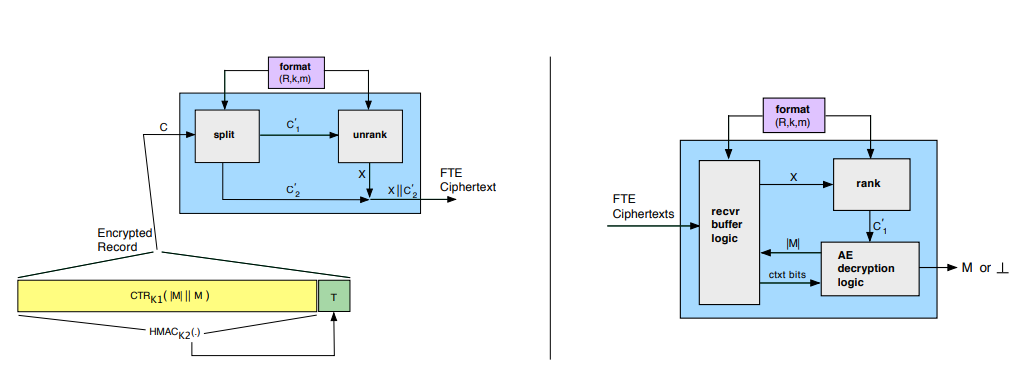
\includegraphics[width = 0.8\textwidth]{FTE_record_layer.png}
        \caption{Схема шифрования и дешифрования}
    \end{center}
\end{figure}

\subsection{Отправитель FTE}

Рассмотрим формат $\mathcal{F} = (R, k, M)$.
Пусть $L_k = L(R) \cap \{0, 1\}^k$ - $k$-битный фрагмент $L(R)$,
оторый будем использовать, а $t = \lfloor \log_2(|L_k(R)|) \rfloor$ - емкость фрагмента,
т.е. количество бит, которое можно закодировать с помощью этого фрагмента.

\begin{enumerate}
    \item Первое действие это подготовка зашифрованной записи с помощью ключа K:
          из буфера открытых сообщений берется открытое сообщение $M$, длиной не более $|M| < m$.
    \item Затем формируется открытая текстовая запись, содержащая закодированную длину $|M|$, за которой следует $M$.
          Эта запись шифруется с помощью стандартной схемы аутентинфицированного шифрования (AE) с ключом $K$ и получается шифротекст $C$.
          Предполагается, что $|C|$ определяется только $|M|$, что справедливо для AE, использующихся на практике.
          Дополняем $M$, если требуется, чтобы гарантировать $|C| \geq t$ (условие криптостойкости по Шенону).
          В предложенной реализации используется режим CTR для AES и аутентифицирует полученнный шифротекст с помощью HMAC-SHA256.
    \item Шифротекст $C$ передаётся функции $split$ и добавляется в его внутренний буфер.
          Функция $split$ создаёт две строки, первую передаёт в unrank для форматирования, а вторую передаёт как есть.
          В частности, функция $split$ извлекает до $t + m$ бит (но не менее $t$ бит) из передней части буфера. Эту часть обозначим как $C'$.
          Важно отметить, что $C'$ может быть полным шифротекстом AE, частью одного или содержать биты из нескольких шифротекстов.
    \item Затем разделяет $C'$ на части $C'_1$ и $C'_2$, где $|C'_1| = t$ и $|C'_2| \leq m$.
          Первая часть $C'_1$ отдаётся функции unrank, которая выдаёт форматированную строку $X \in L_k(R)$.
          И наконец, конкатенация $X \| C'_2$ становится шифротекстом FTE отправителя, который может быть передан.
\end{enumerate}

\subsection{Получатель FTE}

Одной из главных проблем здесь является отсутствие явных маркеров для разграничения границ шифротекстов FTE.
Решением этой проблемы является та форма формата, которую была определена ранеее:
для получения шифротекста использовался фиксированный фрагмент $L_k(R)$.

\begin{enumerate}
    \item При появление во входном буффере $k$-бит шифротекста FTE,
          получатель рассматривает их как строку $X \in L_k(R)$ и применяет функцию $rank(X)$ для восстановления $C'_1$ (или выдаётся ошибка, если $X \notin L_k(R)$).
    \item Затем $C'_1$ передаётся в алгоритм расшифровки AE для получения $l = |M|$ и, возможно, некоторых начальных бит сообщения $M$.
          (Эти последние биты сообщения ещё не должны быть переданы на более высокие уровни).
          Следует отметить, что схема аутентифицированного шифрования должна поддерживать возможность инкрементного дешифрования
          и быть устойчивой к атакам, которые могут злоупотреблять использованием поля длины до обеспечения целостности. Режим CTR и HMAC обеспечивают эти свойства.
    \item Учитывая значение $l$, пролучатель теперь знает, сколько ещё бит шифротекста AE ожидается.
          Отсюда он может удалить из входного буфера до $m$ бит шифротекста,
          а затем вернуться в состояние в котором он обрабатывает последующие $k$-бит в буфере в виде строки $L_k(R)$, применяя ранг и т.д.
    \item При получении полного шифротекста AE завешает дешифрование, проверяет целостность шифротекста
          и только теперь освобождает буферизированные биты сообщения.
\end{enumerate}

\subsection{Согласование регулярных выражений}

Уникальной особенностью FTE является возможность быстрого изменения регулярных выражений ``на лету''.
Хотелось бы иметь возможность согласовывать формат, но поскольку в сети все данные, передаваемые по сети,
должны быть отформатированы для прохождения DPI-проверки, согласование регулярных выражений в открытом виде невозможно.
Предлагается решать эту проблема на момент установления TCP-соединения, считая,
что сервер и клиент поддерживают начальный большой набор возможных регулярных выражений.
Т.е. считается, что у клиента сервера есть общий упорядоченный список FTE форматов $(\mathcal{F}_1, \mathcal{F}_2, ..., \mathcal{F}_n)$,
а также что они согласовали свои криптографические ключи вне канала связи.

\begin{enumerate}
    \item Для каждого TCP-соединения клиент выбирает формат FTE $\mathcal{F}_i$ для клиент-серверных сообщений и формат FTE $\mathcal{F}_j$ для сервер-клиентских сообщений.
    \item Затем клиент собирает сообщение $M \leftarrow i \| j$, отмечает его как специальный тип сообщения для согласования,
          используя зарезервированный первый байт открытого текста, кодирует его с помощью $\mathcal{F}_i$ и отправляет на сервер.
    \item Полученное сообщение от клиента сервер перебирает список форматов, пытаясь расшифровать его.
    \item После успешной расшифровки сервер определяет необходимые форматы и использует $\mathcal{F}_i$
          для клиент-серверных сообщений и $\mathcal{F}_j$ для сервер-клиентских сообщений.
    \item Сервер завершает сеанс, отвечая клиенту сообщением с типом завершения согласования.
\end{enumerate}

Можно усовершенствовать обычную реализацию на стороне приемника за счёт наличия процедуры rank,
которая содержит специальные проверки на быстрое завершение разбора, когда строка была отранжирована, но не принята конечным автоматом.
Это позволяет автомату быстро исключить определенные автоматы, и тем самым обеспечить поддержку десятков автоматов.

\section{Заключение}

В данной работе была дана классификация систем обхода блокировок. Самыми перспективными оказались системы на основе туннелирования и мимикрии.
Рассмотрены существующие инструменты обфускации соединений, которые применяются в Tor. Среди них подробно рассмотрен FTE,
так как оно обладает теми же выразительными свойствами, что и сами DPI системы.

Что могло ещё быть рассмотрено в рамках данной темы:
\begin{enumerate}
    \item Методы детектирования атак протокольного туннелирования.
    \item Описание работы DNS-Morph, который основан на obfs4 и DNS-туннелировании.
    \item Усовершествование FTE за счёт HTTP-туннелирования. FTE использовался бы для мимикрии файлов,
          которые передаются через полезную нагрузку HTTP, что усложнило бы работу DPI-систем.
\end{enumerate}

\newpage

\begin{thebibliography}{9}
\bibitem {} Mihir Bellare, Thomas Ristenpart, Phillip Rogaway, Till Stegers. Format-Preserving Encryption.
\bibitem {} Kevin P. Dyer, Scott E. Coull, Thomas Ristenpart, Thomas Shrimpton. Protocol Misidentification Made Easy.
\bibitem {} Rami Ailabouni, Orr Dunkelman, Sara Bitan. DNS-Morph UDP-Based Bootstrapping Protocol For Tor.
\bibitem {} Piyush Sharma, Devashish Gosain. Camoufler Accessing The Censored Web By Utilizing Instant Messaging.
\bibitem {} Zhonghang Sui, Hui Shu, Fei Kang, Yuyao Huang, Guoyu Huo. A Comprehensive Review of Tunnel Detection on Multilayer Protocols.
\end{thebibliography}


\end{document}
